\documentclass[11pt,a4paper]{article}
\usepackage{amsmath,amsthm,amsfonts,amssymb,amscd}
\usepackage{enumerate} 
\usepackage{physics}
\usepackage{enumerate}
\usepackage{fancyhdr}
\usepackage{hyperref}
\usepackage{graphicx}
\usepackage{xurl}

%---- added for warning box
\usepackage{tcolorbox}
%----- end of "added for warning box"


\hypersetup{colorlinks,
    linkcolor=blue,
    citecolor=blue,      
    urlcolor=blue,
}

\oddsidemargin0.1cm 
\evensidemargin0.8cm
\textheight22.7cm 
\textwidth15cm \topmargin-0.5cm

\newtheorem{theorem}{Theorem}[section]
\newtheorem{lemma}[theorem]{Lemma}
\newtheorem{corollary}{Corollary}
\newtheorem{proposition}{Proposition}

\theoremstyle{definition}
\newtheorem{remark}{Remark}
\newtheorem{definition}{Definition}
\newtheorem{observation}{Observation}
\newtheorem{note}{Note}
\newtheorem{hope}{Hope}
\newtheorem{warning}{Warning}
\newtheorem{problem}{Problem}
\newtheorem{fear}{Fear}
\newtheorem{question}{Question}

\newcommand{\Z}{\mathbb{Z}}
\newcommand{\R}{\mathbb{R}}
\newcommand{\C}{\mathbb{C}}
\newcommand{\Q}{\mathbb{Q}}
\newcommand{\A}{\mathbb{A}}

\usepackage{listings, listings-rust}
\usepackage{xcolor}

\definecolor{codegreen}{rgb}{0,0.6,0}
\definecolor{codegray}{rgb}{0.5,0.5,0.5}
\definecolor{codepurple}{rgb}{0.58,0,0.82}
\definecolor{backcolour}{rgb}{0.95,0.95,0.92}

\lstdefinestyle{mystyle}{
    backgroundcolor=\color{backcolour},   
    commentstyle=\color{codegreen},
    keywordstyle=\color{magenta},
    numberstyle=\tiny\color{codegray},
    stringstyle=\color{codepurple},
    basicstyle=\ttfamily\footnotesize,
    breakatwhitespace=false,         
    breaklines=true,                 
    captionpos=b,                    
    keepspaces=true,                 
    numbers=left,                    
    numbersep=5pt,                  
    showspaces=false,                
    showstringspaces=false,
    showtabs=false,                  
    tabsize=2
}

\lstset{style=mystyle}

\newcommand{\MultiSet}{\mathrm{MultiSet}}
\newcommand{\len}{\mathrm{len}}
\newcommand{\din}{\texttt{d\_in}}
\newcommand{\dout}{\texttt{d\_out}}
\newcommand{\Relation}{\texttt{relation}}
\newcommand{\X}{\mathcal{X}}
\newcommand{\Y}{\mathcal{Y}}
\newcommand{\U}{\texttt{U}}
\newcommand{\True}{\texttt{True}}
\newcommand{\False}{\texttt{False}}
\newcommand{\clamp}{\texttt{clamp}}
\newcommand{\function}{\texttt{function}}
\newcommand{\float}{\texttt{float }}
\newcommand{\questionc}[1]{\textcolor{red}{\textbf{Question:} #1}}

\newcommand{\silvia}[1]{{ {\color{blue}{(silvia)~#1}}}}
\newcommand{\grace}[1]{{ {\color{purple}{(grace)~#1}}}}
\newcommand{\connor}[1]{{ {\color{teal}{(connor)~#1}}}}

\newcommand{\todo}{{\textcolor{red}{TODO }}}


\title{Privacy Proofs for OpenDP: Bounded Sum with Known $n$}
\author{S\'ilvia Casacuberta, Grace Tian, Connor Wagaman}
\date{Version as of \today~(UTC)}

\begin{document}

\maketitle

\tableofcontents

\bigskip

\begin{tcolorbox}
\begin{warning}[Proof only applies to integer types]
Please note that this proof only applies for bounded sums calculated on integers. Specifically, the user-specified type \texttt{T} (more details on \texttt{T} can be found in Section \ref{sec:pseudocode}) must be an integer type, such as \texttt{u32} or \texttt{i64}.

Other types should be used with caution; for example, we know that the current implementation does not work for floats.
\end{warning}
\end{tcolorbox}

\section{Versions of definitions documents}
\label{sec:versioned-docs}

When looking for definitions for terms that appear in this document, the following versions of the definitions documents should be used.

\begin{itemize}
    \item \textbf{Pseudocode definitions document:} This proof file uses the version of the pseudocode definitions document available as of September 23, 2021, which can be found at \href{https://github.com/opendp/whitepapers/blob/pseudocode-defns/pseudocode-defns/pseudocode_defns.pdf}{this link} (archived \href{https://github.com/opendp/whitepapers/blob/cfab535367f592c1242ab880002cc726822506a0/pseudocode-defns/pseudocode_defns.pdf}{here}).
    
    \item \textbf{Proof definitions document:} This file uses the version of the proof definitions document available as of September 23, 2021, which can be found at \href{https://github.com/opendp/whitepapers/blob/proof-defns/proof-defns/proof_defns.pdf}{this link} (archived \href{https://github.com/opendp/whitepapers/blob/f43bf7056a5fd3b6f7b4bb77d451eafa042fe8f7/proof-defns/proof_defns.pdf}{here}). 
\end{itemize}

\section{Algorithm Implementation}
\subsection{Code in Rust}
The current OpenDP library contains the transformation \texttt{make\_bounded\_sum\_n} implementing the bounded sum function with known $n$. This is defined in lines 29-49 of the file \texttt{mod.rs} in the Git repository\footnote{Updated on September 20, 2021.} (\url{https://github.com/opendp/opendp/blob/8bbb0fab1da9b86c50235a36d7026189be43b1ab/rust/opendp/src/trans/sum/mod.rs#L29-L49}).

%\begin{figure}[ht]
    %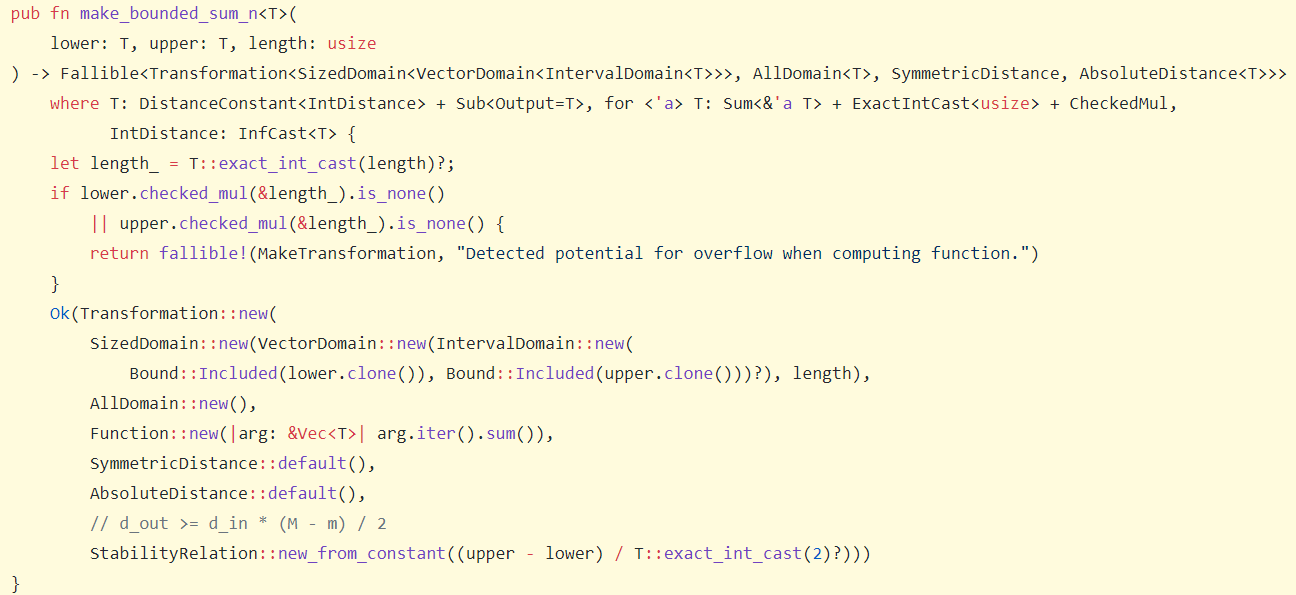
\includegraphics[width=15cm]{bounded_sum_2.png}
    %\centering
    %\label{fig:code}
%\end{figure}

\begin{lstlisting}[language = Rust]
pub fn make_sized_bounded_sum<T>(
    size: usize, bounds: (T, T)
) -> Fallible<Transformation<SizedDomain<VectorDomain<BoundedDomain<T>>>, AllDomain<T>, SymmetricDistance, AbsoluteDistance<T>>>
    where T: DistanceConstant<IntDistance> + Sub<Output=T>, for <'a> T: Sum<&'a T> + ExactIntCast<usize> + CheckedMul + CheckNull,
          IntDistance: InfCast<T> {
    let size_ = T::exact_int_cast(size)?;
    let (lower, upper) = bounds.clone();
    if lower.checked_mul(&size_).is_none()
        || upper.checked_mul(&size_).is_none() {
        return fallible!(MakeTransformation, "Detected potential for overflow when computing function.")
    }
    Ok(Transformation::new(
        SizedDomain::new(VectorDomain::new(
            BoundedDomain::new_closed(bounds)?), size),
        AllDomain::new(),
        Function::new(|arg: &Vec<T>| arg.iter().sum()),
        SymmetricDistance::default(),
        AbsoluteDistance::default(),
        StabilityRelation::new_from_constant((upper - lower) / T::exact_int_cast(2)?)))
}
\end{lstlisting}

\subsection{Pseudocode}
\label{sec:pseudocode}
We present pseudocode represenation of the \texttt{MakeBoundedSumN} function below. The necessary definitions for the pseudocode can be found in Section \ref{sec:versioned-docs}.

\subsubsection*{Preconditions}
To ensure the correctness of the output, we require the following preconditions:

\begin{itemize}
    \item \textbf{User-specified types:}
    \begin{itemize}
        \item Variable \texttt{n} must be of type \texttt{usize}.
        \item Type \texttt{T} must have traits \texttt{DistanceConstant(IntDistance)}, \texttt{TotalOrd}, \texttt{CheckNull}, \texttt{CheckedMul}, \texttt{CheckedSub}, \texttt{Sum(Output=T)}, \texttt{Sub(Output=T)},  and \texttt{ExactIntCast(usize)}.
        \item \texttt{IntDistance} must have trait \texttt{InfCast(T)}. (Note that this bullet point is not needed in this proof, but it is needed in the code so a hint can be constructed; otherwise a binary search would be needed to construct the hint.)
        \item Variables \texttt{U} and \texttt{L} must be of type \texttt{T}, and we must have $\texttt{L} \leq \texttt{U}$.

\end{itemize}
\end{itemize}

\subsubsection*{Postconditions}
\begin{itemize}
    \item Either a valid \texttt{Transformation} is returned or an error is returned.
\end{itemize}

\begin{lstlisting}[language=Python, escapechar=|]
def MakeBoundedSumN(L: T, U: T, n: usize):
    input_domain = SizedDomain(VectorDomain(IntervalDomain(L, U)), n)
    output_domain = AllDomain(T)|\label{code:output-domain}|
    input_metric = SymmetricDistance()|\label{code:symm-dist}|
    output_metric = AbsoluteDistance(T)|\label{code:abs-dist}|
    
    n_ = exact_int_cast(n, T)|\label{code:exact-int-cast}|
    if checked_mul(L, n_).is_none or checked_mul(U, n_).is_none: |\label{code:no-overflow-sum}|
        raise Exception('Potential overflow') |\label{line:max}|
    
    def relation(d_in: u32, d_out: T) -> bool: |\label{line:rel}|
        d_in_ = inf_cast(d_in, T)
        if checked_mul(2, d_out).is_none or checked_mul(d_in_, U-L).is_none|\label{code:checked-arith-1}|
            or checked_sub(U, L).is_none:|\label{code:checked-arith-2}|
            raise Exception('Overflow occurs in the stability relation')
        return 2*d_out >= d_in_ * (U - L)
    
    def function(data: Vec[T]) -> T: |\label{line:fn}|
        return sum(data) |\label{line:sum}|
    
    return Transformation(input_domain, output_domain, function, input_metric, output_metric, stability_relation = relation)
\end{lstlisting}

\section{Current discrepancies between the Rust implementation and the proof}

To guarantee the correctness of the proof, we highlight the discrepancies that this pseudocode and proof have with respect to the actual Rust implementation:
\begin{itemize}
    \item The pseudocode implementation makes the necessary checks with \texttt{checked\_mul} to avoid overflow issues when computing the stability relation. 
    \item The Rust code does not impose the restriction for \texttt{T} to be an integer type. As noted in the initial warning, the current stability relation only guarantees correctness for integer types.
    \item The Rust code uses the stability relation $\dout \geq \din \cdot (\texttt{U}-\texttt{L})/2$ instead of the relation found in the pseudocode, namely $2\cdot \dout \geq \texttt{inf\_cast}(\din, \texttt{T})\cdot (\texttt{U}-\texttt{L})$. There is already a PR to resolve this discrepancy: \url{https://github.com/opendp/opendp/pull/315}.
    \item The Rust code does not check for possible overflow errors when performing the arithmetic operation $\texttt{U}-\texttt{L}$, whereas the current pseudocode includes a \texttt{checked\_sub} for it.
    \item The Rust code does not include an \texttt{inf\_cast} in the stability relation, which is necessary for type correctness, but there is already a PR that resolves this discrepancy: \url{https://github.com/opendp/opendp/blob/493fe87273adca3294551faa927039b755c1756e/rust/opendp/src/trans/sum/mod.rs#L65-L94}.
    \item The previous PR also includes the new user-specified type trait \texttt{InfDiv}, which the current pseudocode does not include.
\end{itemize}

These changes will soon be applied to the Rust code. The pseudocode also uses the variable \texttt{n} instead of Rust's \texttt{size}, which is more conventional for proof writing.

\section{Proof}
\subsection{Symmetric Distance}
\begin{theorem}
\label{thrm:privacy-proof}
    For every setting of the input parameters \texttt{(L, U, n)} to \texttt{MakeBoundedSumN} such that the given preconditions hold, \texttt{MakeBoundedSumN} raises an exception (at compile time or run time) or returns a valid transformation with the following properties:
    \begin{enumerate}
        \item \textup{(Appropriate output domain).} For every element $v$ in \texttt{input\_domain}, $\function(v)$ is in \texttt{output\_domain}.
        
        \item \textup{(Domain-metric compatibility).} The domain \texttt{input\_domain} matches one of the possible domains listed in the definition of \texttt{input\_metric}, and likewise \texttt{output\_domain} matches one of the possible domains listed in the definition of \texttt{output\_metric}.
        
        \item \textup{(Stability guarantee).} For every pair of elements \texttt{v}, \texttt{w} in \texttt{input\_domain} and for every pair $(\din, \dout)$,  where $\din$ has the associated type for \texttt{input\_metric} and $\dout$ has the associated type for \texttt{output\_metric}, if \texttt{v}, \texttt{w} are $\din$-close under \texttt{input\_metric} and $\texttt{relation}(\din, \dout) = \True$, then \texttt{function(v)}, \texttt{function(w)} are $\dout$-close under \texttt{output\_metric}.
    \end{enumerate}
\end{theorem}

\begin{proof}
    \textbf{(Part 1 -- appropriate output domain).} For \texttt{MakeBoundedSumN}, this is corresponds to showing that for every vector \texttt{v} in \texttt{SizedDomain(VectorDomain(IntervalDomain (L, U)), n)}, where \texttt{L} and \texttt{U} have type \texttt{T}, \texttt{function(v)} belongs to \texttt{AllDomain(T)}.
    
    The output correctness follows from the overflow check done through the \texttt{checked\_mul} function on line \ref{line:max} and from the type signature of \texttt{function} as defined on line \ref{line:fn}.
    
    % \connor{I recommend including a discussion here of the \texttt{exact\_int\_cast}. You should demonstrate that the checked mul thing does the check that we want it to. In doing that demonstration, it is important to show that the number of rows \texttt{n} is not underestimated. The exact\_int\_cast ensures that. \texttt{exact\_int\_cast} is needed to ensure that our checked mul checks the thing we want it to check}
    
    % \connor{I will add an explanation of the use of exact\_int\_cast in line \ref{code:exact-int-cast} here.}
    
    The check for overflow ensures that \texttt{function(v)} is contained within the interval \texttt{[get\_min\_value(T), get\_max\_value(T)]}, and hence prevents any overflow from occurring in calculating the return value on line \ref{line:sum}. The check for overflow works in the following way: first, the size of the vector on which we are taking the bounded sum is \texttt{exact\_int\_cast}ed to a value \texttt{n\_} of type \texttt{T} so that we can work with it (if \texttt{n} it cannot be casted exactly -- for example, if \texttt{n} falls outside the range of values representable by type \texttt{T} -- a cast error will be returned; we know that the \texttt{exact\_int\_cast} will work because \texttt{T} has trait \texttt{ExactIntCast(usize)}). Then, we do a \texttt{checked\_mul} that multiplies \texttt{n\_} and \texttt{L}, and which returns \texttt{None} if the result overflows. Because \texttt{checked\_mul(L,n\_)} is the minimum possible sum we could get, and because \texttt{checked\_mul(U,n\_)} is the maximum possible sum we could get, we know that if neither of these cases will result in overflow, then no overflow will occur at any step in our calculation of the final answer. If \texttt{None} is returned by the \texttt{checked\_mul}, indicating that overflow can occur, then line~\ref{line:max} will raise an exception for potential overflow.
    
    The type signature on \texttt{function(v)} automatically enforces that \texttt{function(v)} has return type \texttt{T} and hence is in \texttt{AllDomain(T)}, which is set on line \ref{code:output-domain} as the \texttt{output\_domain}. Since the Rust code successfully compiles, by the type signature the appropriate output domain property must hold. Otherwise, the code will raise an exception for incorrect input type.
    \end{proof}
    
    \begin{proof}
    \textbf{(Part 2 -- domain-metric compatibility).} For \texttt{MakeBoundedSumN}, proving this part corresponds to showing that \texttt{SizedDomain(VectorDomain(IntervalDomain (L, U)), n)} is compatible with \texttt{SymmetricDistance()} (see line \ref{code:symm-dist}), and that \texttt{AllDomain(T)} is compatible with \texttt{AbsoluteDistance(T)} (see line \ref{code:abs-dist}).
    The former follows directly from the list of compatible domains in the definition of symmetric distance, as described in the pseudocode definitions document in Section \ref{sec:versioned-docs}. The latter follows directly from the list of compatible domains in the definition of absolute distance, as described in the pseudocode definitions document in Section \ref{sec:versioned-docs}. 
    \end{proof}
    
    
    % Flag on the comptaibility of metrics and domains
    
    % \iffalse
    % \smallskip
    
    % \connor{Problem with current stability guarantee. Ideas copied from Slack, so sorry about the formatting.}
    
    % \color{teal}
    
    % I think if we did ((upper - lower) + 1) / 2, then we'd be in good shape. This is because we want to make sure that our d\_out is big enough (for privacy, it's worse to have d\_out small). Because upper and lower are both ints, the difference will be an int.

    % Current relation: Assume (U-L) divisible by 2. Then we're good. Now assume (U-L) not divisible by 2. Then \texttt{(U-L)/2} < (U-L)/2, where \texttt{(U-L)/2} is done on a computer. Uh-oh.

    % "+1" relation: Assume (U-L) divisible by 2. Then \texttt{((U-L)+1)/2} = (U-L)/2, so we're good. Now assume (U-L) not divisible by 2. Then ((U-L)+1) divisible by 2, so ((U-L)+1)/2 is greater than the true (U-L)/2, so we're good.
    
    
    % Another idea is to do something like ``if upper-lower is odd, do the +1 strategy. If it's even, use the original relation''. Not sure if this conditional structure has any implementation-based advantages or disadvantages, but it'll be a tight bound.
    
    % \color{black}
    % \connor{End of notes about the current stability guarantee.}
    
    % \silvia{We ended up concluding that the best option is to move the constant to the other side -- namely, $2 \cdot \dout \geq \din \cdot (\texttt{U}-\texttt{L})$}.
    % \fi
    
    Before beginning the proof of the third part of theorem \ref{thrm:privacy-proof}, we provide a lemma.
    
    \begin{lemma}[Pseudocode guarantee to arithmetic guarantee]
    \label{lemma:pseudo-to-arith}
    Whenever \texttt{2*d\_out >= inf\_cast(d\_in, T)*(U-L)} holds, then, when performing true arithmetic, $\dout \geq \din * (U-L)/2$ also holds.
    \end{lemma}
    
    
    \begin{proof}
    Assume that we have $\texttt{2*d\_out >= inf\_cast(d\_in, T)*(U-L)}$. Note that our checked arithmetic operations in lines \ref{code:checked-arith-1} and \ref{code:checked-arith-2} have the effect of enforcing that $\texttt{(U-L)} = (U-L)$. The operation \texttt{inf\_cast(d\_in,T)} has the property that $\texttt{inf\_cast(d\_in,T)} \geq \texttt{d\_in}$. The checked arithmetic also ensures that \texttt{inf\_cast(d\_in,T)*(U-L)} is exact, so we have the guarantee that $\texttt{inf\_cast(d\_in,T)*(U-L)}\geq \din*(U-L)$. The checked arithmetic also ensures that \texttt{2*d\_out} does not overflow, which has the effect of ensuring that $\texttt{2*d\_out} = 2*\dout$.
    
    Therefore, we have $\texttt{2*d\_out} = 2*\dout \geq \texttt{inf\_cast(d\_in,T)*(U-L)}\geq \din*(U-L)$, so we have $2*\dout\geq \din*(U-L)$. We now divide both sides by 2; since we are working with true arithmetic now, the inequality $\dout\geq \din*(U-L)/2$ is clearly true under our assumption that $\texttt{2*d\_out >= inf\_cast(d\_in, T)*(U-L)}$. This completes our proof that, if $\texttt{2*d\_out >= inf\_cast(d\_in, T)*(U-L)}$, then $\dout \geq \din * (U-L)/2$.
    \end{proof}
    
    \begin{proof}
    \textbf{(Part 3 -- stability guarantee).} 
    Throughout the stability guarantee proof, we can assume that $\texttt{function(v)}$ and $\texttt{function(w)}$ are in the correct output domain, by the \textit{appropriate output domain property} shown above. 
    
    % \textbf{}
    
    % Since by assumption \texttt{relation(d\_in, d\_out) = True}, by the \texttt{MakeBoundedSumN} stability relation (as defined in line~\ref{line:rel} in the pseudocode), we have that \texttt{2 *  d\_out >= inf\_cast(d\_in, T) * (U-L)}. This is equivalent to the stability relation $\dout \geq \texttt{inf\_cast}(\din, T)\cdot (U-L)/2$, which is the one we will show in the proof, except that we avoid any possible integer rounding errors by multiplying by 2 instead of dividing. We will also drop the \texttt{inf\_cast} in the rest of the proof, given that it ensures the correct type of $\din$ but does not affect the bounds of the relation. 

    % trying to rewrite the paragraph above this
    
    Since by assumption \texttt{relation(d\_in, d\_out) = True}, by the \texttt{MakeBoundedSumN} stability relation (as defined in line~\ref{line:rel} in the pseudocode), we have that \texttt{2 *  d\_out >= inf\_cast(d\_in, T) * (U-L)}. Therefore, by Lemma \ref{lemma:pseudo-to-arith}, we also have that $\dout \geq \din * (U-L)/2$.
    
    
    % We show that, if we prove that 
    % This is equivalent to the stability relation $\dout \geq \texttt{inf\_cast}(\din, T)\cdot (U-L)/2$, which is the one we will show in the proof, except that we avoid any possible integer rounding errors by multiplying by 2 instead of dividing. We will also drop the \texttt{inf\_cast} in the rest of the proof, given that it ensures the correct type of $\din$ but does not affect the bounds of the relation. 
    
    We now show that, if $\dout \geq \din * (\texttt{U}-\texttt{L})/2$, then \texttt{function(v)}, \texttt{function(w)} are $\dout$-close under \texttt{output\_metric}.

    
    % end of trying to rewrite the paragraph above this
    
    Moreover, note in the statement of theorem \ref{thrm:privacy-proof} that $\texttt{v}, \texttt{w}$ are assumed to be $\din$-close. By the definition of the symmetric distance metric in the proof definitions document linked in Section \ref{sec:versioned-docs}, this is equivalent to stating that $d_{Sym}(v, w) = |\MultiSet(v) \Delta \MultiSet(w)| \leq \din$. Further, applying the histogram notation,\footnote{Note that there is a bijection between multisets and histograms, which is why the proof can be carried out with either notion. For further details, please consult the proof definitions document in Section \ref{sec:versioned-docs}.} it follows that
    \[
        d_{Sym}(v, w) = \lVert h_{v} - h_{w}\rVert_1 = \sum_z |h_v(z) - h_w(z)| \leq \din.
    \]
    We now want to show that
    \[
        d_{Abs}(\function(v), \function(w)) \leq d_{Sym}(v, w) \cdot \dfrac{U-L}{2}.
    \]
    
    % start of reorganization
    
    To show that $d_{Abs}(\function(v), \function(w)) \leq d_{Sym}(v, w) \cdot \frac{U-L}{2}$, we will use the three lemmas described in the section ``The path property of symmetric distance on sized domains" from Section 5.2 in the proof definitions document (linked in section \ref{sec:versioned-docs}). By Lemma 5.7 in the proof definitions document (linked in Section \ref{sec:versioned-docs}), which is applicable to \texttt{MakeBoundedSumN} because \texttt{input\_domain} is a a sized domain and \texttt{input\_metric} is symmetric distance, it suffices to show the following: For all vectors $x, y \in$ \texttt{input\_domain} such that $d_{Sym}(x, y) = 2$, it follows that 
    \[
    d_{Abs}(\texttt{function}(x), \texttt{function}(y)) \leq U-L.
    \]
    
    By Lemma 5.6 from the proof definitions document (linked in Section \ref{sec:versioned-docs}), we know that vectors $x, y$ only differ on one element, given that, by assumption, $d_{Sym}(x, y) = 2$.
    
    Let $x = (x_1,x_2,\ldots,x_n)$ and $y = (y_1,y_2,\ldots,y_n)$. The fact that we have $d_{Sym}(x, y) = 2$ tells us that there is some vector $z = (z_1,z_2,\ldots,z_n)$ such that, for all $i\neq j$, we have $x_i=z_i$ (and that for $j$, we have $x_j \neq z_j$), and such that $\MultiSet(z)=\MultiSet(y)$. This construction of $z$ gives us the following equalities: $|\sum_i(x_i) - \sum_i(y_i)| = |\sum_i(x_i)-\sum_i(z_i)| = |\sum_i(x_i-z_i)| = |x_j-z_j|$. Because, in a worst-case scenario, the difference between $x_j$ and $z_j$ is the difference between the upper bound $U$ and lower bound $L$, we see that $|x_j-z_j|\leq |U-L| = U-L$ (with the last equality from the fact that $U\geq L$), which is what we wanted to show.
    
    (Note that line \ref{code:no-overflow-sum} prevents overflow from occurring in our calculation of the \texttt{sum} of a vector, and that working with data of an integer type means that we will not experience rounding at any point in our calculation of the \texttt{sum} of a vector. This has the effect that, for all vectors \texttt{v}, we will have $\texttt{sum(v)} = \sum_i(\texttt{v}_i)$.)
    
    
    % end of reorganization
    
    
    The fact that $d_{Abs}(\function(v), \function(w)) \leq d_{Sym}(v, w) \cdot \dfrac{U-L}{2}$ implies that
    \begin{equation}\label{eq:abs1}
        d_{Abs}(\function(v), \function(w)) \leq d_{Sym}(v, w) \cdot \dfrac{U-L}{2} \leq \din \cdot \dfrac{U-L}{2},
    \end{equation}
    and by the stability relation this will imply that
    \begin{equation}\label{eq:abs2}
        d_{Abs}(\function(v), \function(w)) \leq \dout,
    \end{equation}
    as we want to see. 
\end{proof}

% \textbf{Using the path property (adjacent pairs approach)}

% To show that $d_{Abs}(\function(v), \function(w)) \leq d_{Sym}(v, w) \cdot \frac{\texttt{U-L}}{2}$, we will use the three lemmas described in the section ``The path property of symmetric distance on sized domains" from Section 5.2 in the proof definitions document (linked in section \ref{sec:versioned-docs}). By Lemma 5.7 in the proof definitions document (linked in section \ref{sec:versioned-docs}), which is applicable to \texttt{MakeBoundedSumN} because \texttt{input\_domain} is a a sized domain and \texttt{input\_metric} is symmetric distance, it suffices to show the following: For all vectors $x, y \in$ \texttt{input\_domain} such that $d_{Sym}(x, y) = 2$, it follows that 
% \[
% d_{Abs}(\texttt{function}(x), \texttt{function}(y)) \leq \texttt{U} - \texttt{L}.
% \]
% By Lemma 5.6 from the proof definitions document (linked in section \ref{sec:versioned-docs}), we know that vectors $x, y$ only differ on one element, given that, by assumption, $d_{Sym}(x, y) = 2$.

% Let $x = (x_1,x_2,\ldots,x_n)$ and $y = (y_1,y_2,\ldots,y_n)$. The fact that we have $d_{Sym}(x, y) = 2$ tells us that there is some vector $z = (z_1,z_2,\ldots,z_n)$ such that, for all $i\neq j$, we have $x_i=z_i$ (and that for $j$, we have $x_j \neq z_j$), and such that $\MultiSet(z)=\MultiSet(y)$. This construction of $z$ gives us the following equalities: $|\sum_i(x_i) - \sum_i(y_i)| = |\sum_i(x_i)-\sum_i(z_i)| = |\sum_i(x_i-z_i)| = |x_j-z_j|$. Because, in a worst-case scenario, the difference between $x_j$ and $z_j$ is the difference between the upper bound $\texttt{U}$ and lower bound $\texttt{L}$, we see that $|x_j-z_j|\leq |\texttt{U}-\texttt{L}| = \texttt{U}-\texttt{L}$ (with the last equality from the fact that $\texttt{U}\geq \texttt{L}$), which is what we wanted to show.

% Finally, we remark that line \ref{code:no-overflow-sum} prevents overflow from occurring in our calculation of the \texttt{sum} of a vector, and that working with data of an integer type means that we will not experience rounding at any point in our calculation of the \texttt{sum} of a vector. As a result, for all vectors \texttt{v}, we will have $\texttt{sum(v)} = \sum_i(\texttt{v}_i)$.


% Wlog, let this different element be the $k$-th element of $x$ and $y$, where $x_k = \alpha$, $y_k = \beta$ with $\alpha \neq \beta$.\footnote{The first element of a vector is indexed by 0.} Then,
% \[
%     d_{Abs}(\texttt{function}(x), \texttt{function}(y)) = |\texttt{function}(x) - \texttt{function}(y)| = 
% \]
% \[
%     = \Big|\sum_{i=0}^{\texttt{n}-1}x_i - \sum_{i=0}^{\texttt{n}-1}y_i\Big| = 
%     \Big|\sum_{i=0}^{\texttt{n}-1}x_i - \sum_{i=0}^{\texttt{n}-1}z_i\Big| = \Big| \sum_{i=0}^{\texttt{n}-1} (x_i - z_i) \Big| = |0 + (x_j - z_j)| \leq |\texttt{U-L}| = \texttt{U-L},
% \]
% since \texttt{U} $\geq$ \texttt{L}.

% We remark that because we do not have overflows and have an integer type, the sums are computed exactly, and so $\MultiSet(z)=\MultiSet(y)$ implies $\sum_i z_i = \sum_i y_i$. For example, this is not true for floating point types.

% commented out the below per the comment at https://github.com/opendp/whitepapers/pull/5#discussion_r714428139. Feel free to restore.

% Therefore, applying Lemma 5.7 from \href{https://www.overleaf.com/project/60d214e390b337703d200982}{``List of definitions used in the proofs"}, it follows that \texttt{function} is $($\texttt{U-L}$)/2$-stable. By definition, this implies that for any $v, w \in$ \texttt{input\_domain},
% \[
%     d_{Abs}(\texttt{function}(v), \texttt{function}(w)) \leq d_{Sym}(v, w) \cdot (\texttt{U-L})/2.
% \]
% Lastly, by Equations~\ref{eq:abs1} and \ref{eq:abs2} this implies that
% \[
%     d_{Abs}(\function(v), \function(w)) \leq \dout,
% \]
% as we want to prove.

%\silvia{Flag: this will be updated to the more general notion of path property (through shortest path metric on a graph), but this matches the current version of the proofs document.}

\end{document}
